\documentclass{article} % For LaTeX2e
\usepackage{iclr2016_conference,times}
\usepackage{hyperref,algorithm,algpseudocode,array,tabularx,multirow,caption,subcaption,amsfonts,url,verbatim,enumitem,amsmath,graphicx}
\usepackage{url}

\title{Fast Parallel SAME Gibbs Sampling on \\ General Discrete Bayesian Networks}

\author{Daniel Seita, Haoyu Chen \& John Canny \\
Computer Science Division \\
University of California, Berkeley \\
Berkeley, CA 94720, USA \\
\texttt{\{seita,haoyuchen,canny\}@berkeley.edu}
}

% The \author macro works with any number of authors. There are two commands used to separate the
% names and addresses of multiple authors: \And and \AND.
%
% Using \And between authors leaves it to \LaTeX{} to determine where to break the lines. Using \AND
% forces a linebreak at that point. So, if \LaTeX{} puts 3 of 4 authors names on the first line, and
% the last on the second line, try using \AND instead of \And before the third author name.
%
% ICLR requires electronic submissions, processed by \url{http://arxiv.org}. See ICLR's website for
% more instructions.
% 
% If your paper is ultimately accepted, the statement {\tt {\textbackslash}iclrfinalcopy} should be
% inserted to adjust the format to the camera ready requirements.
% 
% The format for the submissions is a variant of the NIPS format.  Please read carefully the
% instructions below, and follow them faithfully.

\newcommand{\fix}{\marginpar{FIX}}
\newcommand{\new}{\marginpar{NEW}}

%\iclrfinalcopy % Uncomment for camera-ready version

\begin{document}

\maketitle

\begin{abstract}
A fundamental task in machine learning and related fields is to
perform inference on Bayesian networks. Since exact inference takes
exponential time in general, a variety of approximate methods are
used.  Gibbs sampling is one of the most accurate approaches and
provides unbiased samples from the posterior but it has historically
been too expensive for large models. In this paper, we present an
optimized, parallel Gibbs sampler whose performance matches
approximate methods, and which is several orders of magnitude faster
than current Gibbs samplers.  Our Gibbs sampler is GPU-accelerated,
heavily parallelized, and uses state replication (SAME or State
Augmented Marginal Estimation) to decrease convergence time. We find
that SAME in general improves parameter estimate quality while it
accelerates convergence.  Experiments on both synthetic and real data
show that our Gibbs sampler is substantially faster than the state of
the art sampler, JAGS, without sacrificing accuracy. Our ultimate
objective is to introduce the Gibbs sampler to researchers in many
fields to expand their range of feasible inference problems.
\end{abstract}




\section{Introduction}\label{sec:intro}

In many machine learning applications, the user has a distribution
$P(X,Z \mid \Theta)$ where $X$ is observed data, $Z$ is hidden
(latent) data, and $\Theta$ represents the model parameters. The goal
is generally to find an optimal $\Theta$ with respect to $X$, while
marginalizing out $Z$. To represent these problems, it is common to
use graphical models.  Here we focus on discrete-state models,
so node transitions are characterized by set of conditional
probability tables (CPTs). Each CPT represents a local probability
distribution $\Pr(X_i \mid X_{\pi_i})$ where $X_i$ is a random
variable, and $X_{\pi_i}$ represents its set of parent nodes in the
graph. We denote the full set of CPTs as $\Theta$.  In general, the
network state is partially observed $\mathcal{D} = \{\xi_1, \ldots,
\xi_m\}$, where $\xi_i$ is an $n$-dimensional vector with assignments
to the $n$ variables of the graph, or ``N/A'' to indicate missing
data. We assume that the structure of the Bayesian network --- its
nodes and edges --- is known in advance, but not the set of
observations. This form allows us to represent latent and well as
observed states, but also observations on an arbitrary
(sample-dependent) subset of those states.

% should discuss MC-EM which is the closest to us
Well-known strategies for parameter estimation with partially observed
data include Expectation-Maximization~\citep{EMpaper} and variations
of gradient ascent~\citep{Thiesson95}.  Parameter estimation using
these methods marginalizing over missing states which typically
dominates performances. Using Monte-Carlo methods for marginalization
leads to the MC-EM methods~\citep{MC-EM}.

For parameter estimation with a Gibbs sampler, we sample both latent
states and parameters from $P(Z,\Theta|\mathcal{D})$.  For the case of
discrete node states, $Z$ follow multinomial distributions while the
$\Theta$ are Dirichlet. Gibbs sampling is widely used in machine
learning but has seen limited use on large datasets.  It is typically
orders of magnitude slower than approximate methods such as {\bf
  should list approx methods here, e.g.  from the KDD paper}. In a
recent result,~\citet{SAME2015} showed that by combining the State
Augmented Monte Carlo (SAME) technique~\citep{SAME2002} with Gibbs
sampling, one can match the speed of approximate methods while
obtaining higher quality estimates. But that paper was restricted to
Latent Dirichlet Allocation and similar models.  In this paper, we
build upon that result by presenting a SAME Gibbs sampler for general
discrete Bayesian networks. The contributions of this paper are

\begin{itemize}[noitemsep]
    \item A more general Gibbs sampler using SAME sampling with improved convergence and better-quality MAP or ML parameter
      estimates over standard samplers.
    \item We parallelize the sampler which provides acceleration on both CPU and GPU
      hardware.
    \item The sampler maintains only model-related state and processes data out-of-memory
      so it can scale to very large datasets (either from disk or network storage).
\end{itemize}

We benchmark our sampler versus a state of the art Gibbs sampler,
JAGS~\citep{JAGS2003}, and find that our Gibbs sampler is multiple
orders of magnitude faster. The throughput and scalability of the
sampler (nodes processed per second) is competitive with special
purpose methods while maintaining the accuracy of Gibbs sampling.


\section{Related Work}\label{sec:related_work}

The problem of Bayesian inference for graphical models is  well-studied (~\citet{Koller2009}
and~\citet{Wainwright2008} covers recent approximate and MCMC methods). Gibbs sampling has proved to
be one of the most important practical techniques for large models. Collapsed samplers are widely
used for LDA and related models~\citep{Griffiths_Steyvers}, parallelism have been improved using
color groups~\citep{Gonzalez2011}, and approximate, uncoordinated parallelism has been shown to give
good results in practice~\citep{Johnson2013}.  Gibbs sampling has been applied to large-scale
databases in~\citep{Zhang2013}.
% guys, you should compare your throughput with that paper. 

Recently, Graphics Processing Units (GPUs) have proved valuable for deep learning, and are used in
most toolkits including Theano \citep{Theano2012}, CAFFE ~\citep{jia2014caffe} and Torch
\citep{Torch}. The Augur probabilistic programming language~\citep{Augur2014}, which generates
inference code for Bayesian networks, demonstrates the importance of combining GPU code with extra
parallelism introduced from exploiting conditional independence assumptions.
% Why is augur discussed here? 

The result most directly related to our paper, as briefly mentioned in Section~\ref{sec:intro}, is
one that shows how the addition of SAME to a GPU-accelerated Gibbs sampler can be very fast for
Latent Dirichlet Allocation and the Chinese Restaurant Process~\citep{SAME2015}. In that paper, they
explored the application of SAME to graphical model inference on modern hardware, and showed that
combining SAME with factored sample representation (or approximation) gives throughput competitive
with the fastest symbolic methods, but with potentially better quality. We extend that result by
implementing a general-purpose Gibbs sampler that can be applied to arbitrary discrete graphical
models.





\section{Fast Parallel SAME Gibbs Sampling}\label{sec:same}

SAME is a variant of MCMC where one artificially replicates latent state to create distributions that
concentrate themselves on the global modes~\citep{SAME2002}. It is an efficient way of performing
MAP estimation in high-dimensional spaces when needing to integrate out a large number of variables.
Given a distribution $P(X,Z\mid \Theta)$, to estimate the most likely $\Theta$ based on the data
$(X,Z)$ using SAME, one would define a new joint $Q$:
\begin{equation}\label{eq:same}
Q(X,\Theta,Z^{(1)},\ldots,Z^{(m)}) = \prod_{j=1}^m P(X,\Theta,Z^{(j)})
\end{equation}
which models $m$ copies of the distribution tied to the same set of parameters $\Theta$, which in
our case forms the set of Bayesian network CPTs. This new distribution $Q$ is proportional to a
\emph{power} of the original distribution, so $Q(\Theta \mid X) \propto (P(\Theta \mid X))^m$. Thus,
it has the same optima, including the global optimum, but its peaks are sharpened~\citep{SAME2002}.
Note that as $m$ increases, SAME approaches Expectation-Maximization~\citep{EMpaper} since the
distribution would peak at the value corresponding to the maximum likelihood estimate.

We argue that SAME is beneficial for Gibbs sampling because it helps
to reduce excess variance derived from discrete sample quantization.
It is important, however, not to set the SAME replication factor $m$
too high, which reduces sampling to EM and may lead to poor local
optima. Instead, since the replication factor is formally equivalent
to a temperature control, it can be used to anneal the sampler to a
low-variance, high-quality parameter estimate.


% \textbf{Daniel: I am really confused about what I should include for this section. I feel like this
%just repeats a lot of the SAME description. It might be necessary to do that, but do we have an idea
% on what we want to discuss?}




\section{Implementation of SAME Gibbs Sampling}\label{sec:implementation}

\begin{figure}[t]
\centering
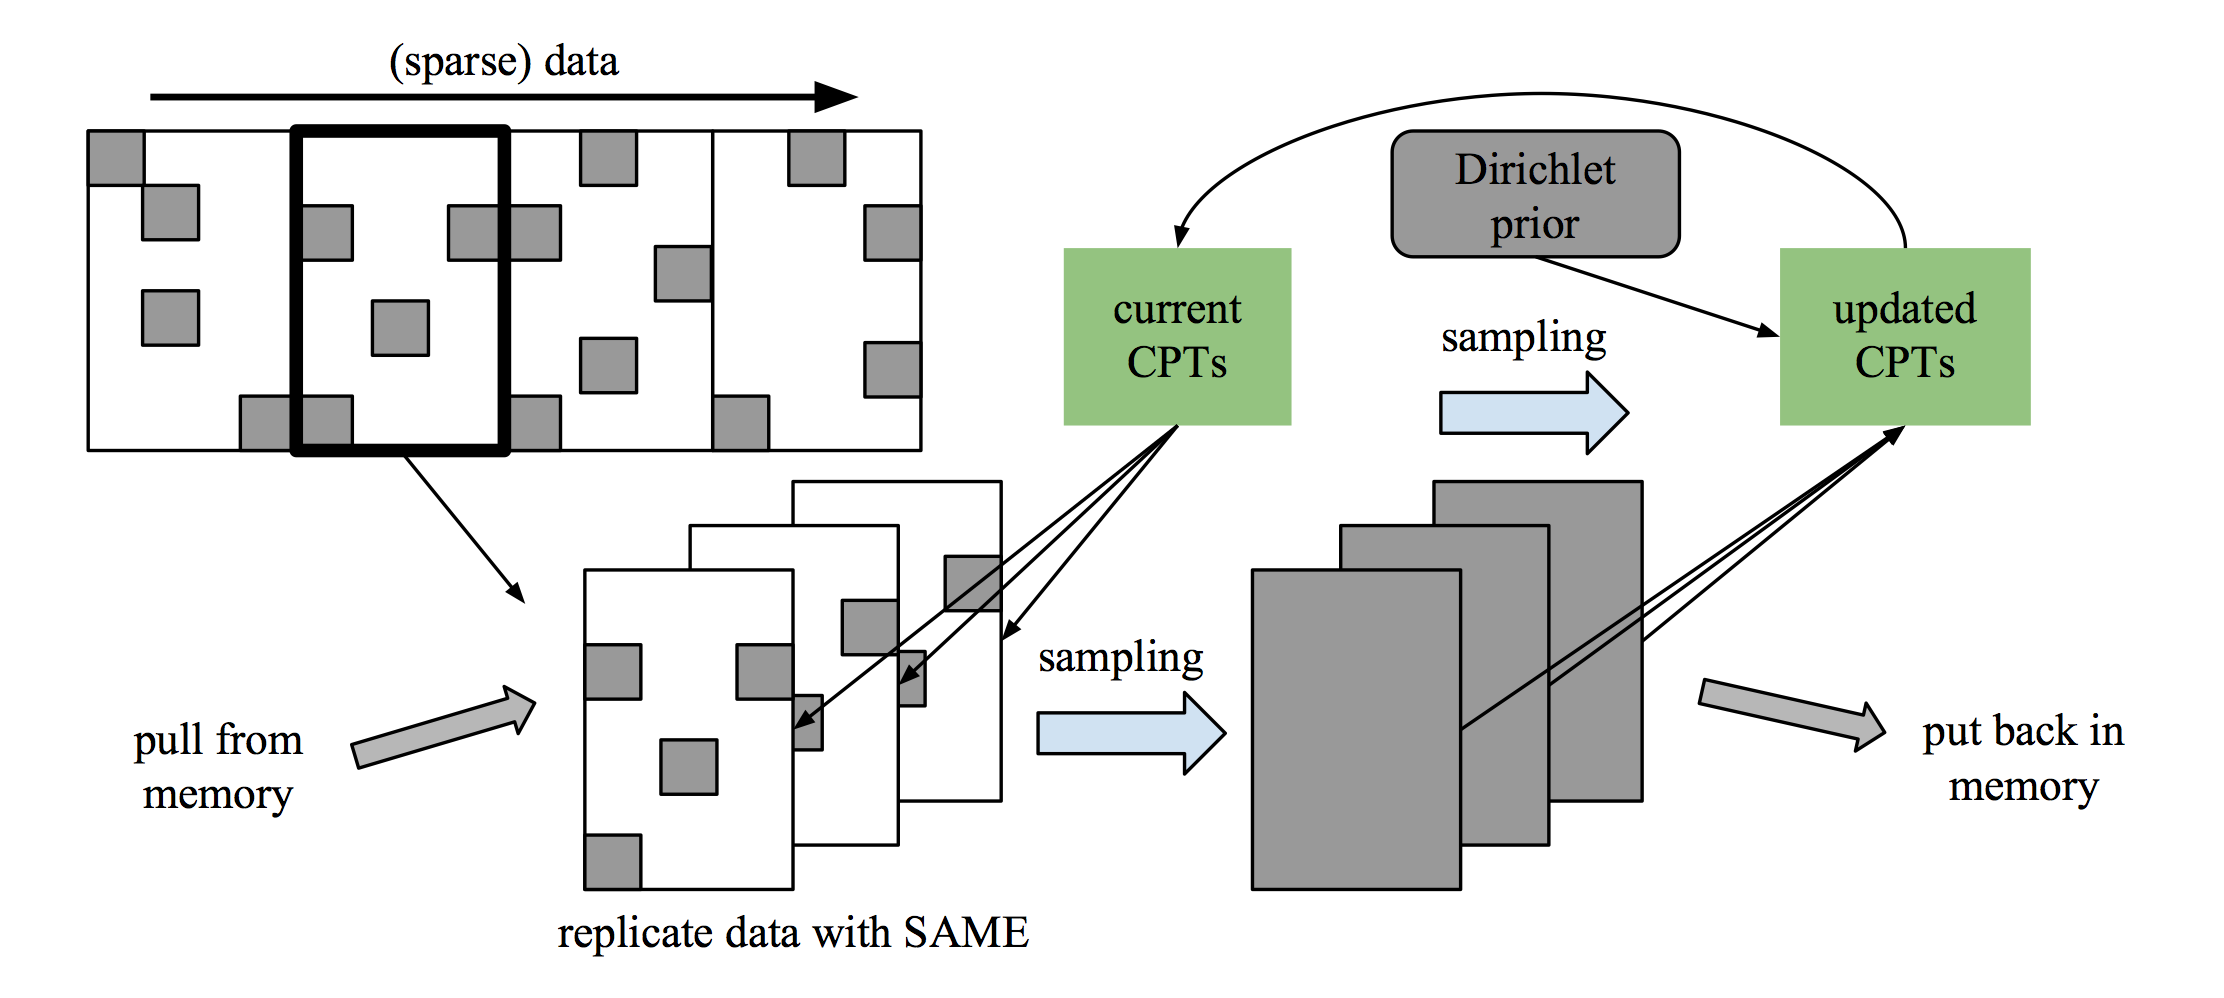
\includegraphics[width=0.75\textwidth]{fig_BIDMach_final}
\caption{This visualizes our Gibbs sampler at work. The original data is split into four
mini-batches of equal sizes (for caching purposes), with each having some known data (shaded gray)
and unknown data (white). For each mini-batch, the sampler replicates the data three times ($m=3$),
samples the unknown values, and then uses those with the prior to update its estimate of the CPTs.}
\label{fig:BIDMach}
\end{figure}

Our Gibbs sampler is implemented as part of the open-source BIDMach library~\citep{bidmach} for
machine learning.  Figure~\ref{fig:BIDMach} shows a visualization of how it works on a large dataset.
Our sampler expects a data matrix (typically sparse), with rows representing variables and columns
representing cases. BIDMach divides data into same-sized \emph{mini-batches} and iterates through
them to update parameters. If there are $M$ minibatches in the entire dataset, we maintain a moving
sum of the state counts for the $M$ most-recently processed minibatches. Updating this average requires 
us to maintain the state counts for each minibatch from the last iteration. We subtract these from
the total state counts before adding in the updated counts for this minibatch from the current iteration.
\footnote{For larger
datasets, this state is not saved and instead the counts are maintained using an exponential moving sum. Thus the memory require scales only with model size, not dataset size.}

Our Gibbs sampler is augmented with SAME. Consequently, if $m$ is the SAME parameter, for each
mini-batch our sampler forms $m$ copies of the known data.  Then, it performs Gibbs sampling to fill
in the missing data in each copy of the mini-batch using the current CPTs.  These sampled results
are combined with an adjustable Dirichlet prior and the current CPTs to form a set of discrete
counts, which form the Dirichlet parameters to update (explicitly sample) the CPTs. 

There are several optimizations used to improve performance.  First, Since
storage allocation is very expensive on GPUs and their memory is
limited on GPUs (3-12 GB is typical), BIDMach use a matrix caching
strategy to reuse memory for matrices of the same
dimensions.

Second Graphical structure and SAME-replicated states for a particular
color group are fused into large matrices to maximize parallelism and
hide GPU-kernel overhead.

As mentioned in Section~\ref{sec:related_work}, we further parallelize Gibbs sampling in an
exact manner via chromatic partitioning. In Bayesian networks, nodes $u$ and $v$ are independent
conditioned on a set of variables $\mathcal{C}$ if $\mathcal{C}$ includes at least one variable on
every path connecting $u$ and $v$ in the \emph{moralized graph} of the network, which is the graph
formed by connecting parents and dropping edge orientations.

Suppose there is a $k$-coloring of the moralized graph such that each vertex is assigned one of $k$
colors and adjacent vertices have different colors. Denote $\mathcal{V}_c$ the set of variables
assigned color $c$ where $1 \leq c \leq k$. One can sample sequentially from $\mathcal{V}_1$ to
$\mathcal{V}_k$, where within each color group, it samples all the variables in parallel. This
parallel sampler corresponds exactly to the execution of a sequential scan Gibbs sampler for some
permutation over the variables and will converge to the desired distribution because variables
within one color group are independent to each other given all the other variables. Finding the
optimal coloring of a general graph is NP-complete, but efficient heuristics for balanced graph
coloring perform well in many problems.




% Daniel: be sure to reference data correctly! Call it "Koller", "Synthetic MOOC", or "Real MOOC".
\section{Evaluating our Gibbs Sampler}\label{sec:experiments}

We benchmark our Gibbs sampler based on one synthetic and one real dataset. We compare it with
JAGS~\citep{JAGS2003}, which is the most popular and efficient tool for Bayesian inference, and also
uses Gibbs sampling as the primary inference algorithm. 

% We could not find another general-purpose
% software package that substantially outperformed JAGS. % I don't think we need to reference BNT.
% That's not specific enough. There are comparisons on the web between JAGS and other tools showing
% its as fast as anything else. You should cite them. 

For all JAGS experiments and for CPU benchmarks for BIDMach, we use a
single computer with an Intel Core Xeon processor with eight cores and
2.20 GHz clock speed (E5-2650 Sandy Bridge). The computer has 64 GB of
CPU RAM. We used a different machine with NVIDIA Titan X GPU for the
GPU experiments (since the CPU characteristics of this second machine
do not affect performance while using the GPU).

\subsection{Synthetic ``Koller'' Data}\label{ssec:koller_data}

\begin{figure}[t]
\centering
\begin{subfigure}{.5\textwidth}
  \centering
  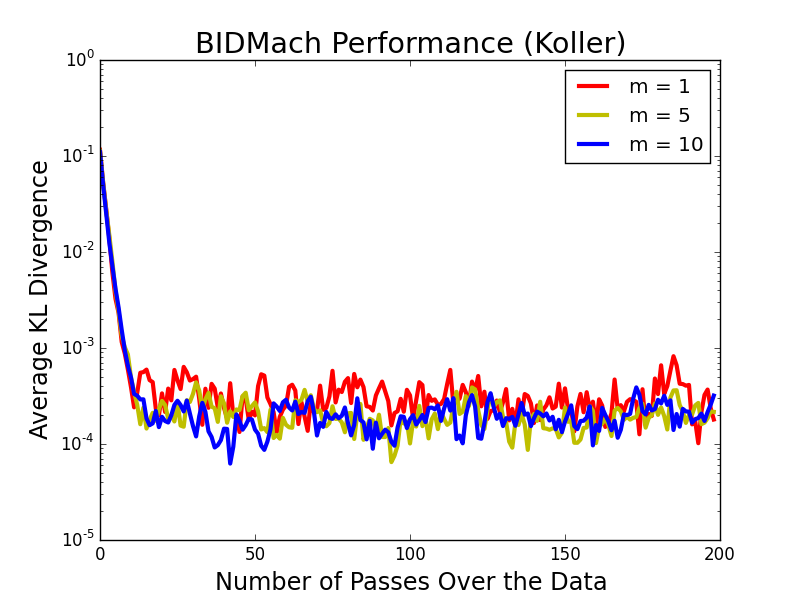
\includegraphics[width=0.9\linewidth]{fig_kldiv_koller_mb4_gpu}
  \caption{The $KL_{\rm avg}$ from BIDMach.}
  \label{fig:kl_bidmach}
\end{subfigure}%
\begin{subfigure}{.5\textwidth}
  \centering
  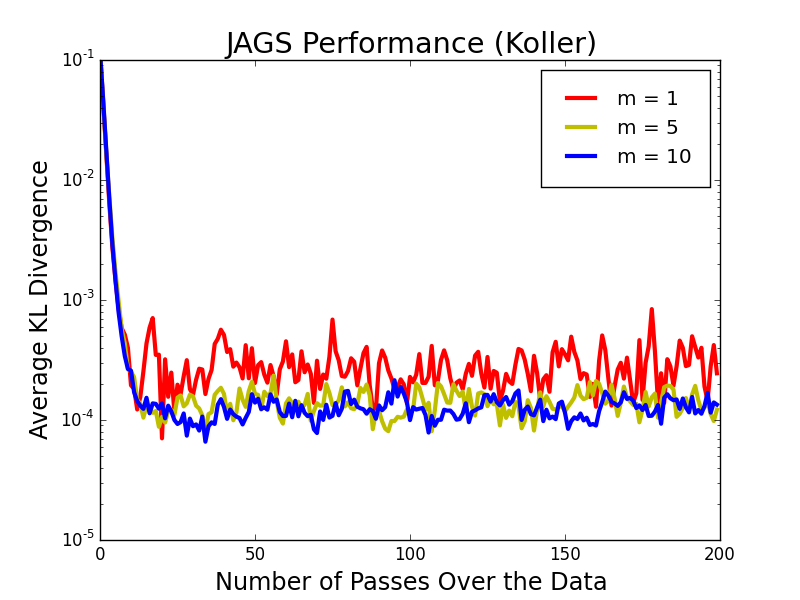
\includegraphics[width=0.9\linewidth]{fig_kldiv_50perc_jags}
  \caption{The $KL_{\rm avg}$ from JAGS.}
  \label{fig:kl_jags}
\end{subfigure}
\caption{Plots of our $KL_{\rm avg}$ curves as a function of the iteration, on Koller data (these
must be viewed in color). Both BIDMach and JAGS converge to the true CPTs quickly, but JAGS appears
to benefit more from the extra data replication with SAME parameters $m=5$ and $m=10$.}
\label{fig:first_set}
\end{figure}

% BIDMach (CPU) vs JAGS for the Koller data. This one only has 50k columns now!
% BIDMach settings: 25k batch size, 200 iterations, 777 seed.  We do get gflops with BIDMach, so we
% can include them if desired, but the runtime is the more interesting thing we want to compare.
% Perhaps we should use total seconds, rather than per iteration? It's easier to understand.
% Also, opts.updateAll = true because we should be updating after each mini-batch.
%
% Here are the BIDMach CPU (not GPU!) results ON BITTER, with extra values if we can get more JAGS results:
%
% Time=8.7060 secs, gflops=0.84 (m=1)
% Time=15.4930 secs, gflops=0.94 (m=2)
% Time=29.7660 secs, gflops=1.23 (m=5)
% Time=67.6580 secs, gflops=1.08 (m=10)
% Time=129.7780 secs, gflops=1.13 (m=20)
%
% BIDMach CPU times on STOUT, which is what we actually have to report!
%
% Time=10.6480 secs, gflops=0.69 (m=1)
% Time=15.3780 secs, gflops=0.95 (m=2)
% Time=31.4540 secs, gflops=1.16 (m=5)
% Time=61.1170 secs, gflops=1.20 (m=10)
% Time=122.2520 secs, gflops=1.20 (m=20)
%
% Yeah, a  bit weird that gflops doesn't increase each time ... also, funny how stout is actually
% faster. That works to our *advantage* here!
%
% EDIT: Argh, we may have to re-run this to get times for FOUR mini-batches since that's what I use
% for Fig 2. Results on stout with mini-batch sizes of 12.5k:
%
% Time=11.0200 secs, gflops=0.66 (m=1) + 0.598s initialization
% Time=18.0350 secs, gflops=0.81 (m=2) + 0.612s initialization
% Time=33.0970 secs, gflops=1.10 (m=5) + 0.631s initialization
% Time=62.2550 secs, gflops=1.17 (m=10) + 0.619s initialization
% Time=115.3720 secs, gflops=1.27 (m=20) + 0.660s initialization
%
% Make sure we mention in the paper that we're deliberately handicapping ourselves. EDIT: wait, wow,
% 12500 can even be faster in some cases? Yeah, CPU runtime is tricky, but these are ballparks anyway.
\begin{table}[t]
\small
\caption{BIDMach (CPU) vs. JAGS Runtime on Koller Data}
\label{tab:bidmach_jags_koller}
\begin{center}
\begin{tabular}{ |c|c|c|c|c|c|c| } 
\hline
                         & $m=1$ & $m=2$ & $m=5$ & $m=10$ & $m=20$ \\
\hline \hline
BIDMach Total Time (sec) & 11.6  & 18.6  & 33.7  & 62.9   & 116.0  \\ 
JAGS Total Time (sec)    & 42.0  & 98.2  & 281.2 & 535.0  & 1037.6 \\
\hline
\end{tabular}
\end{center}
\end{table}

We first use synthetic data generated from a small Bayesian network to check correctness
and the use of SAME. The network has five variables: $X_0 = {\rm Intelligence}$, $X_1 =
{\rm Difficulty},$ $X_2 = {\rm SAT}$, $X_3 = {\rm Grade}$, and $X_4 = {\rm Letter}$. The directed
edges are $\mathcal{E} = \{(X_0, X_2), (X_0, X_3), (X_1,X_3), (X_3,X_4)\}$, where $(X_i,X_j)$ means
an arrow points from $X_i$ to $X_j$.  Variable $X_3$ is ternary, and all others are binary. This
network models a student taking a class, and considers ability metrics (Intelligence and SAT score),
the class difficulty, and the student's resulting grade, which subsequently affects the quality of a
letter of recommendation. This network, along with the true set of CPTs, is from Chapter 3
of~\citet{Koller2009}. Due to the name of the author, we call this the ``Koller'' data to
distinguish it from the MOOC data we use in~(\ref{ssec:mooc_data}).

To generate the data, we use the standard technique of forward sampling, where $X_i$ gets sampled
based on the true distributions from~\citet{Koller2009}, which depends on $X_i$'s parents (if any).
We repeat this to get 50,000 samples, then randomly hide 50\% of the data points. The goal is to
apply Gibbs sampling to estimate the CPTs that generated the data. Note that BIDMach can handle
millions of samples but we use only 50,000 for benchmarking with JAGS.

To evaluate our Gibbs sampler, we compute the average KL Divergences of all the distributions in the
set of CPTs, denoted as $KL_{\rm avg}$.  For two distributions $p(x)$ and $q(x)$, the KL divergence
is $\sum_x p(x) \log(p(x)/q(x))$, summing over $x$ such that $q(x) > 0$.  In the Koller data, there
are eleven probability distributions that form the set of CPTs. For example, $X_4$ ``contributes''
three distributions: $\Pr(X_4 \mid X_3 = 0), \Pr(X_4 \mid X_3 = 1)$, and $\Pr(X_4 \mid X_3 = 2)$,
where $X_3$ (the parent) is fixed. For this network, we have $KL_{\rm avg} = \frac{1}{11}
\sum_{i=1}^{11} p_i(x) \log(p_i(x)/q_i(x))$, where $q_i$ is the distribution our sampler estimates
and $i$ is some arbitrary indexing notation. We do not use the KL Divergence of the full joint
distribution $P(X_1,X_2,X_3,X_4,X_5)$ since with high-dimensional data (e.g., the MOOC data
in~(\ref{ssec:mooc_data})), computing the full joint is intractable and we wish to facilitate
comparisons across different datasets.

Figures~\ref{fig:kl_bidmach} and~\ref{fig:kl_jags} plot the $KL_{\rm avg}$ metric for the student
data using BIDMach and JAGS, respectively with three SAME factors (note the log scale). The plots
indicate that the $KL_{\rm avg}$ for BIDMach and JAGS reach roughly the same values, with a slight
advantage to JAGS, though this is amplified because of the log scale. In practice, the difference
would be indistinguishable to humans. For instance, with $m=1$, the average difference between a
random number in the sampled CPT and its corresponding number in the true CPT for BIDMach and JAGS,
respectively, is 0.0039 and 0.0043. Thus, both BIDMach and JAGS will sample CPTs that are accurate
to two/three decimal places.

For BIDMach, we tuned the mini-batch size to be 12,500. Using a smaller size means that, for a fixed
number of passes, we tend to get faster convergence, but this often comes with slower runtime per
iteration. In addition, we observed that increasing $m$ results in CPT estimates that more closely
match the true CPTs. The red curves (i.e., $m=1$) for Figures~\ref{fig:kl_bidmach}
and~\ref{fig:kl_jags} generally correspond to worse $KL_{\rm avg}$ than the respective yellow and
blue curves, with the difference more noticeable for JAGS. Also, going from $m=5$ to $m=10$ seems to
have a negligible benefit.

We further benchmark the speed of our CPU Gibbs sampler with JAGS on this data. For a fair
comparison, we keep our mini-batch size to be 12,500 to match the runs from
Figure~\ref{fig:kl_bidmach}.  Table~\ref{tab:bidmach_jags_koller} shows the total runtime on the
data with different $m$ for 200 passes. We used total runtime because the JAGS API does not enable
us to separate the initialization time from the updating/sampling time. (JAGS spends a substantial
amount of time initializing here since it needs to form a graph, but BIDMach uses matrices and
spends less than one second in initialization.) The results demonstrate that BIDMach is almost four
times faster than JAGS on the original data, and when the SAME parameter increases, the gap widens
(up to a factor of nine with $m=20$).

\subsection{Dynamic Learning Maps ``MOOC'' Data}\label{ssec:mooc_data}

% Daniel: a few things to argue about for the kldiv_synthmooc_gpu_300iter_02b.png figure.
% EDIT: I changed the figure to use the 'bad' starting point.
%   (1) These are in fact the steady states. I ran the BIDMach data for 500 iterations, and the
% graphs level out at where they level out (i.e., the 2.2% and 5% data look like they're going up *a
% little* but then they have another smooth decrease, etc.).
%   (2) Also note the random starting point. This data's CPT is very even (lots of 50-50 stuff) so
% JAGS will usually pick a good starting point, but BIDMach is completely random (which is what I
% used here). In the 25% data, the steady state is roughly 0.007. JAGS seems like it can get there
% in 7-8 iterations, while it seems like we take roughly 3-3.5 times that much. When we initialize
% with a smoother prior, we tend to get convergence in about 2-2.5 times as many iterations (which
% one can argue we should be using anyway).
%   (3) Also consider the batch size. We are using 2184 so we have two mini-batches. More frequent
% updates with smaller batch sizes can get the convergence down to about 1.5-2 times as many
% iterations, but at an unacceptable extra time cost (i.e., the time would go up by double if we
% halve the batch size, but the convergence time is not halved when we do that), so we felt from
% informal tuning that two mini-batches was appropriate.
%   (4) Finally, we can tune the SAME parameter. With a smooth prior (adding 10 to the starting
% CPT), and also with SAME = 20, and a batch size of 500, I was able to get convergence in 10
% iterations, roughly matching JAGS. We should say that in reality, the cost tradeoff is somewhat
% unacceptable and we will stick with what we have here (i.e., losing a factor of 3 in converge rate
% per iteration). The fact that BIDMach is fast and easily tunable means that tuning can and should
% be done to get high quality models. We should mention that we do not know why JAGS converges
% faster, and analyzing the source code did not help.
\begin{figure}[t]
\centering
\begin{subfigure}{.5\textwidth}
  \centering
  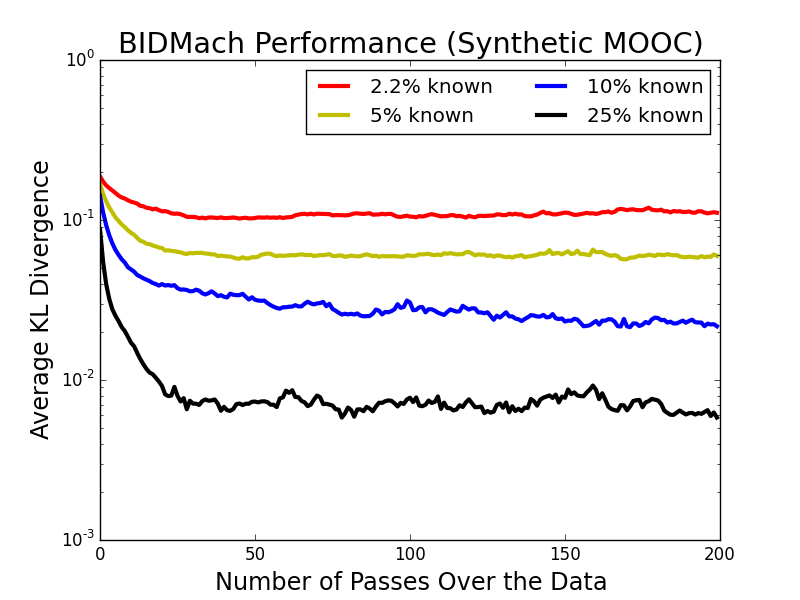
\includegraphics[width=0.9\textwidth]{fig_diff_sparsity_bidmach}
  \caption{The $KL_{\rm avg}$ from BIDMach.}
  \label{fig:kl_bidmach_mooc}
\end{subfigure}%
\begin{subfigure}{.5\textwidth}
  \centering
  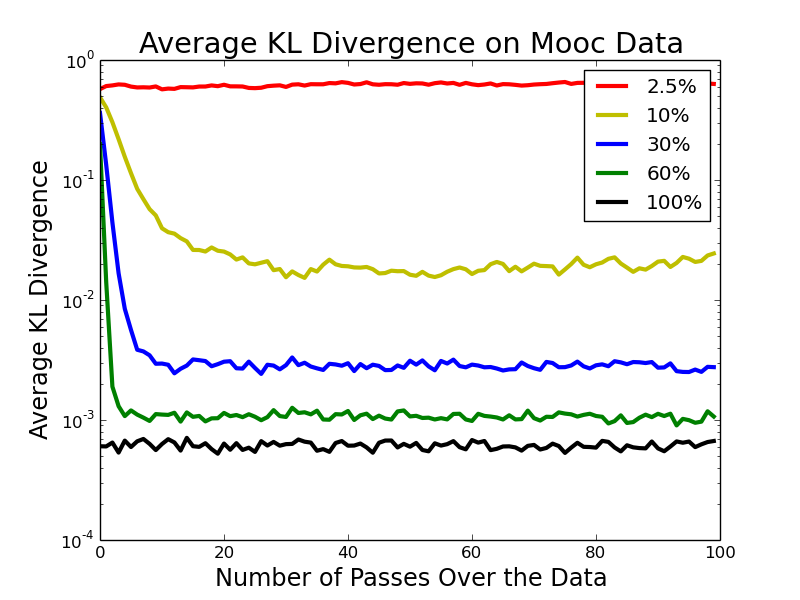
\includegraphics[width=0.9\textwidth]{fig_diff_sparsity_jags}
  \caption{The $KL_{\rm avg}$ from JAGS.}
  \label{fig:kl_jags_mooc}
\end{subfigure}
\caption{Plots of our $KL_{\rm avg}$ curves as a function of the iteration, on Synthetic MOOC Data
with different sparsity levels (these must be viewed in color).}
\label{fig:second_set}
\end{figure}

\begin{figure}[t]
\centering
\begin{subfigure}{.5\textwidth}
  \centering
  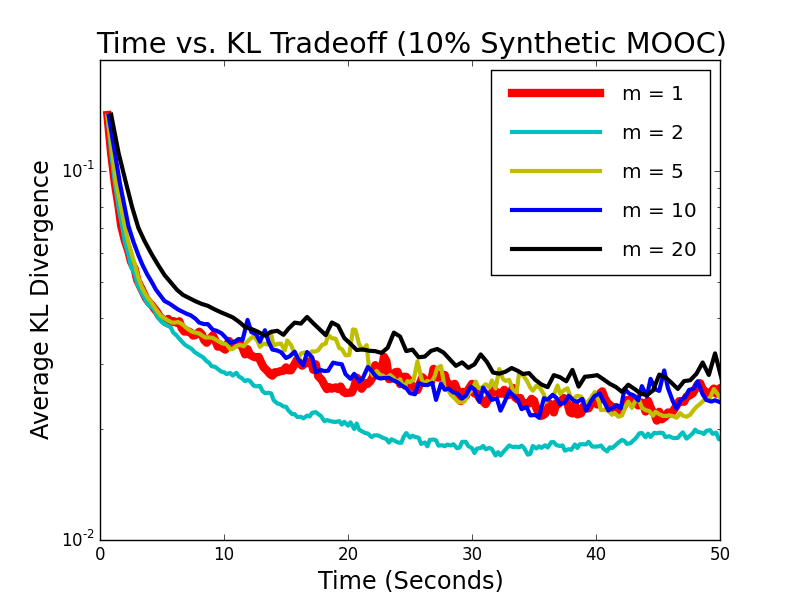
\includegraphics[width=0.9\textwidth]{fig_kltime_tradeoff_mooc}
  \caption{The $KL_{\rm avg}$ from BIDMach.}
  \label{fig:mooc_kl}
\end{subfigure}%
\begin{subfigure}{.5\textwidth}
  \centering
  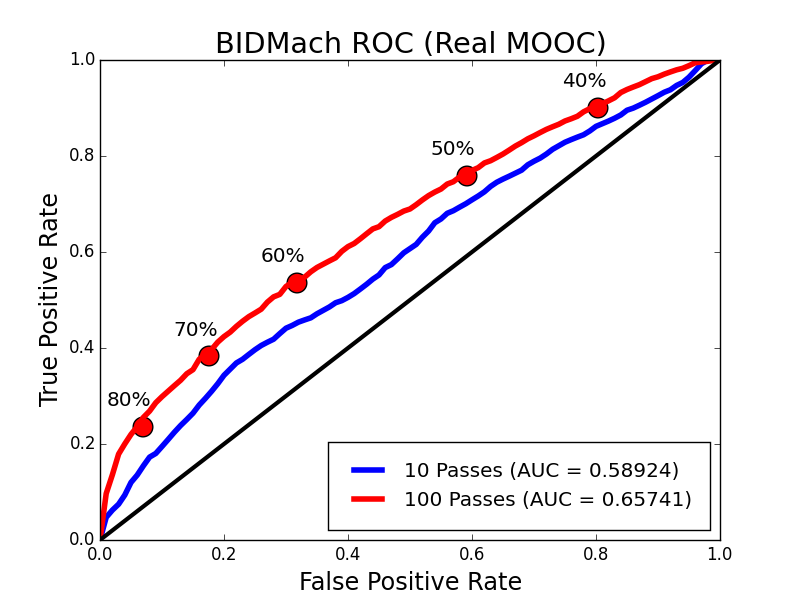
\includegraphics[width=0.9\textwidth]{fig_bidmach_real_mooc_roc_curve_v2}
  \caption{MOOC data ROC curve.}
  \label{fig:mooc_accuracy}
\end{subfigure}
\caption{Some more results ($KL_{\rm avg}$ and ROCs) of our sampler on Synthetic/Real MOOC data.}
\label{fig:third_set}
\end{figure}


We now benchmark our code on a Bayesian network with a nation-wide examination dataset from the
Dynamic Learning Maps (DLM) project\footnote{URL: \url{http://dynamiclearningmaps.org/}. There is no
official paper reference for this data.}. The data contains the assessment (correct or not) of
student responses to questions from the DLM Alternate Assessment System. After preprocessing, there
are 4367 students and 319 questions. Each of the questions is derived from a set of 15 basic
concepts. We encode questions and concepts as variables and describe their relationships with a
Bayesian network from the DLM data. (The 15 concepts are latent variables across all students.) Each
question is a variable with a very high missing value rate.  Our corresponding data matrix, which
has dimensions $(334\times 4367)$, has a 2.2\% sparsity level. The inference task is to learn the
CPTs of the Bayesian network from this extremely sparse data.

We evaluate our sampler using two methods. The first involves running it on the original data until
convergence. Then we use the resulting estimated set of CPTs and sample from that via forward
sampling to generate ``Synthetic MOOC'' data, also of dimension $(334 \times 4367)$. We create
several versions of this data, each with a different fraction of missing data. Then we re-run
BIDMach on these and evaluate the CPTs using the same $KL_{\rm avg}$ metric
from~(\ref{ssec:koller_data}). Computing $KL_{\rm avg}$ involves averaging over 682 distributions
based on the Bayesian network, which has relatively few edges (the most amount of parents any node
has is three).

Figures~\ref{fig:kl_bidmach_mooc} and~\ref{fig:kl_jags_mooc} plot the $KL_{\rm avg}$ for BIDMach and
JAGS, respectively on four different levels of sparsity (note again the log scale). As expected,
BIDMach and JAGS converge to roughly the same $KL_{\rm avg}$. Furthermore, ``denser'' data allows
the Gibbs sampler to get closer to the true CPTs. BIDMach and JAGS start at different $KL_{\rm avg}$
values due to different initializations; JAGS tends to initialize at $50-50$, roughly matching the
real CPTs, while BIDMach initializes randomly.

We also analyze the tradeoffs involved in increasing the SAME factor $m$. While increasing $m$
intuitively (and theoretically) should lead to faster convergence to higher quality parameter
estimates, it is possible that increasing $m$ too much will result in getting stuck in a local
maxima since this is a highly noncovex problem. Figure~\ref{fig:mooc_kl} plots\footnote{The baseline
$m=1$ curve is thicker for readability.} $KL_{\rm avg}$ as a function of total time elapsed. The
$m=2$ curve is clearly better as for a fixed time $t$, it has lower $KL_{\rm avg}$ than $m=1$,
despite how the $m=1$ curve will have had more full passes over the data. Interestingly enough,
$m=5$ results in similar results, and the $m=20$ curve indicates that higher $m$ will not be
beneficial.  We ran the experiment for Figure~\ref{fig:mooc_kl} for 300 seconds and the longer-term
trend was that the $KL_{\rm avg}$ values tended to remain at their 50-second values.

In addition to measuring distance between predicted and actual parameters, we evaluate
the sampler also using its accuracy at predicting missing labels.  We divide the original
data into a training and testing batch so that 80\% of the known data is in training. The training
set is used to update the CPTs. During the testing phase, we sample $n$ times using the current CPTs
without updating them. For each (correct) test state, this yields an unbiased estimate of the correct state
probability. 

% Ach what went wrong? Can we fix this. Otherwise we have an invalid test set
% The training and testing data have 62.8\% and 57.6\% of known data points in the positive class,
% respectively. Due to this imbalance, we do not use raw accuracy as a predictor and instead turn to
We use Receiver Operating Characteristic (ROC) curve to estimate the predictors effectiveness.
Figure~\ref{fig:mooc_accuracy} shows the ROC curves obtained after 10 passes and 100 passes through the data. 
After 100 passes, the ROC has an AUC of 0.65741. 
% that's disturbing. 
% we tested at other points, such as 1000 passes (AUC of 0.63792), but did not find any curve with an AUC exceeding 0.65741, possibly due to overfitting
% after 100 passes. Figure~\ref{fig:mooc_accuracy} also has five labeled dots, from 40\% to 80\%.
% These indicate different decision point cutoffs. For instance, the point labeled at 50\% is the
% point on the ROC curve that corresponds to the decision threshold being positive if we have at least
% 50\% of our samples as positive (out of 500, meaning we need at least 250). The 0\% decision
% threshold (not shown) would correspond to the point $(1,1)$.



\section{Speed and Scalability of Our Sampler on Large Data}\label{sec:scaling_large_data}

% BIDMach (CPU) vs JAGS for the Real MOOC data *replicated*, with SAME=1.
% Batch size: we'll use 2184 (approx 4367/2) to be a fair comparison with previous table with
% Koller, because we usually like to have more than one mini-batch.
%
% Here are the BIDMach CPU (not GPU!) results on BITTER:
%
% Time=36.4890 secs, gflops=1.20 (1x)
% Time=71.5470 secs, gflops=1.22 (2x)
% Time=196.5920 secs, gflops=1.11 (5x)
% Time=387.2260 secs, gflops=1.13 (10x)
% Time=739.8330 secs, gflops=1.18 (20x)
% 
% Here are the CPU BIDMach times on STOUT with the same settings, which is what we report:
%
% Time=38.4290 secs, gflops=1.14 (1x) + 1.06s initialization
% Time=75.0240 secs, gflops=1.17 (2x) + 1.061s initialization
% Time=186.2360 secs, gflops=1.17 (5x) + 1.066s initialization
% Time=358.4780 secs, gflops=1.22 (10x) + 1.125s initialization
% Time=700.2980 secs, gflops=1.25 (20x) + 1.092s initialization
% Time=1436.2930 secs, gflops=1.22 (40x) + 1.115s initialization
%
% Notes on JAGS: we tried with 100x, but it crashed (ran out of memory) on stout, after almost 30
% minutes. And actually, 40% crashed as well. But on stout, BIDMach only uses 11.4% of the memory
% with 40% of the data.
%
% GPU times on bitter:
%
% Time=9.2280 secs, gflops=4.74 (1x) + 1.985 init
% Time=19.1550 secs, gflops=4.56 (2x) + 2.007 init
% Time=46.0210 secs, gflops=4.75 (5x) + 2.095 init
% Time=90.9390 secs, gflops=4.80 (10x) + 1.937 init
% Time=181.8290 secs, gflops=4.80 (20x) + 2.019 init
% Time=363.7390 secs, gflops=4.80 (40x) + 2.127 init
%
\begin{table}[t]
\small
\caption{BIDMach (CPU) vs. JAGS Runtime on (Replicated) Real MOOC Data}
\label{tab:bidmach_jags_realmooc}
\begin{center}
\begin{tabular}{ |c|c|c|c|c|c|c| } 
\hline
                             & 1x    & 2x     & 5x     & 10x     & 20x     & 40x    \\
\hline \hline
GPU BIDMach Total Time (sec) & 11.2  & 21.2   & 48.1   & 92.9    & 183.8   & 365.9  \\ 
CPU BIDMach Total Time (sec) & 39.5  & 76.1   & 187.3  & 359.6   & 701.4   & 1437.4 \\ 
JAGS Total Time (sec)        & 975.2 & 2749.0 & 5830.0 & 18815.0 & 34309.0 & OOM    \\
\hline
\end{tabular}
\end{center}
\end{table}


% This should be in another section. We might consider splitting this in two if we have space. For
% both of these, I chose the largest batch size that we could do m = 50.
%
% Koller Data = (5 x 1,000,000)-dimensional, mini-batch size = 50,000, iterations = 200, seed = 777.
% This is with the sliding, rectangular window of samples, which is *slower* than the moving
% average,  hence we'll get slower gflops. Before, with complete truncation (but an incorrect
% graphical model, technically speaking) we were getting 13.90 for m = 50.
% Final statistics from BIDMach:
% Time=61.4750 secs, gflops=2.38 (m=1)
% Time=71.8440 secs, gflops=4.07 (m=2)
% Time=104.6140 secs, gflops=6.98 (m=5)
% Time=160.8270 secs, gflops=9.08 (m=10)
% Time=265.6820 secs, gflops=11.00 (m=20)
% Time=374.4060 secs, gflops=11.70 (m=30)
% Time=476.0510 secs, gflops=12.27 (m=40)
% Time=591.2360 secs, gflops=12.35 (m=50)
%
% MOOC Data = (334 x 43670)-dimensional, where we replicated the *real* mooc 5x column-wise. Hence,
% RM = Replicated MOOC. Again, this is with the sliding, rectangular window of samples. I was going
% to use 10x, but I would have had to shrink the batch size down to 100 (or even less than that), I
% think because putback requires extra memory or something. So I'm doing 5x, which lets me increase
% the batch size to 400. More advanced GPUs in the future will allow us to run this faster.

% Settings: mini-batch size = 400, SAME is the variable. 200 iterations and 777 seed as usual.
% Total runtimes were:
%
% Time=133.2460 secs, gflops=1.65 (m=1)
% Time=238.3670 secs, gflops=4.58 (m=5)
% Time=308.1950 secs, gflops=7.08 (m=10)
% Time=450.3450 secs, gflops=9.69 (m=20)
% Time=599.5060 secs, gflops=10.92 (m=30)
% Time=750.6940 secs, gflops=11.62 (m=40)
% Time=907.2790 secs, gflops=12.02 (m=50)
%
% Now for the actual table itself EDIT this was the old table. I have a new one now.
%\begin{table}[t]
%\caption{BIDMach (GPU) Runtime vs. GigaFlops on Large Data}
%\label{tab:tradeoff}
%\begin{center}
%\begin{tabular}{ |c|c|c|c|c|c|c|c| } 
%\hline
%               & $m=1$ & $m=5$ & $m=10$ & $m=20$ & $m=30$ & $m=40$ & $m=50$  \\
%\hline \hline
%GigaFlops (K)  & 2.38  & 6.98  & 9.08   & 11.00  & 11.70  & 12.27  & 12.35   \\ 
%Time/Iter (K)  & 0.307 & 0.523 & 0.804  & 1.328  & 1.872  & 2.380  & 2.957   \\
%\hline 
%GigaFlops (RM) & 1.65  & 4.58  & 7.08   & 9.69   & 10.92  & 11.62  & 12.02   \\ 
%Time/Iter (RM) & 0.666 & 1.192 & 1.541  & 2.252  & 2.998  & 3.753  & 4.536   \\
%\hline
%\end{tabular}
%\end{center}
%\end{table}
 
% New table. The Koller data is similar, but the BIDMach data is different.  We're using 30 TIMES
% the data, with a batch size of 1000. For SAME = 10, this uses up 95% of the GPU memory. Times:
%
% Time=488.0840 secs, gflops=2.69 (m=1)
% Time=587.9970 secs, gflops=4.46 (m=2)
% Time=836.1830 secs, gflops=7.83 (m=5)
% Time=1262.6890 secs, gflops=10.37 (m=10)
%
\begin{table}[t]
\small
\caption{BIDMach (GPU) Runtime Per Iteration and GigaFlops on Large Data}
\label{tab:tradeoff}
\begin{center}
\begin{tabular}{ |c|c|c|c|c|c| } 
\hline
               & $m=1$ & $m=2$ & $m=5$ & $m=10$ \\
\hline \hline
GigaFlops (Koller, 1M)               & 2.38  & 4.07  &  6.98  &  9.08  \\ 
Time (sec) / Iteration (Koller, 1M)  & 0.307 & 0.359 &  0.523 &  0.804 \\
\hline
GigaFlops (30x MOOC)              & 2.69  & 4.46  & 7.83  & 10.37   \\ 
Time (sec) / Iteration (30x MOOC) & 2.440 & 2.940 & 4.181 & 6.313   \\
\hline
\end{tabular}
\end{center}
\end{table}

We now discuss the extent to which BIDMach (and JAGS) can scale up to larger datasets in order to
identify the limits of current software. We were unable to obtain anything larger than the MOOC data
from~(\ref{ssec:mooc_data}), so we formed ``larger datasets'' by replicating the MOOC data
horizontally: we took the data matrix and made $n$ copies to get a $(334 \times 4367n)$-dimensional
data matrix. In Table~\ref{tab:bidmach_jags_realmooc}, we report the time per iteration for BIDMach
and JAGS on a variety of replicated data, from the original data (1x) to data replicated 40 times
(40x). For our sampler, we used the same tunable settings (e.g, mini-batch size) as we did in
Figure~\ref{fig:second_set}, to keep our benchmarks consistent. Just as in
Table~\ref{tab:bidmach_jags_koller}, we report total runtime for 200 iterations.

The results indicate that BIDMach holds a clear speed advantage over JAGS, though one must interpret
the results carefully. From Figure~\ref{fig:second_set}, we see that, while BIDMach and JAGS both
eventually converge to similar $KL_{\rm avg}$ values, our sampler takes roughly three times as many
iterations to reach convergence (this is most easily observed on the 25\% data). We can reduce the
number of iterations for BIDMach to reach convergence by reducing the mini-batch size, but our
informal experiments indicated that doing so would result in unacceptable time increases.

Therefore, to determine BIDMach's speed improvements, one would need to divide the JAGS time by
three (roughly). Despite this caveat, our sampler still has a huge performance advantage. With the
original data, BIDMach's advantage is a factor of $(975.2/3)/39.5 \approx 8.23$, and the gap widens
with more data (for 20x, we have an advantage of $(34309.0/3)/701.4\approx 16.31$). We emphasize
that this result is with the CPU only. The GPU version, especially on larger data (e.g., the 20x
data) typically results in another order of magnitude improvement. In terms of memory usage, BIDMach
also outperforms JAGS. BIDMach structures data in matrices, whereas JAGS internally forms a graph.
For the 40x data, JAGS ran out of memory on our 64 CPU RAM machine, whereas BIDMach only used up
11.4\% of the RAM.

It is also worthy to investigate the impact of the SAME parameter $m$, in terms of runtime \emph{and
throughput}, which is measured in GigaFlops (gflops), a billion floating point operations per
second. As the SAME parameter increases, it increases both the throughput (good) and runtime (bad)
by increasing the number of data points in our computations. The results from~\citep{SAME2015}
suggest that increasing $m$ for small values will increase throughput while not costing too much in
runtime.  As one increases $m$ beyond a certain data-dependent value, then SAME ``saturates'' the
algorithm and results in stagnant throughput while significantly increasing runtime.
Figure~\ref{fig:mooc_kl} also raises the question as to whether one really needs a large $m$ in the
first place.

Table~\ref{tab:tradeoff} reports the performance of BIDMach's GPU version (only) on two expanded
datasets with varying $m$. One is the Koller data from~(\ref{ssec:koller_data}), with 50\% of the
data known versus missing, but with \emph{one million} cases. The other is 30x replicated MOOC data.
Table~\ref{tab:tradeoff} reports that BIDMach gets a healthy amount of throughput from the expanded
data (especially the 30x MOOC data), and that increasing $m$ further is a logical possibility.

Finally, we point out that the runtimes in all tables in this paper are listed are in seconds, and
even with large $m$ and a large replication factor, we have barely scratched the limit of our
sampler. In fact, the primary limiting factor of our sampler is not the data itself, but the memory
of the GPU. As we get better and faster GPUs, the performance of our sampler will improve and we
will be able to run it on larger and larger datasets.



\section{Conclusions}\label{sec:conclusions}

We conclude that our Gibbs sampler is much faster than the state of
the art (JAGS) and can be applied to data with hundreds of discrete
variables and millions on instances. We also suggest that SAME can be
beneficial for Gibbs sampling, and that SAME Gibbs sampling should be
the go-to method for researchers who wish to perform inference on
(discrete) Bayesian networks. Future work will explore the application
of our sampler to a wider class of real-world datasets.


\subsubsection*{Acknowledgments}

We thank Yang Gao, Biye Jiang, and Huasha Zhao for helpful discussions.

\bibliography{iclr2016_conference}
\bibliographystyle{iclr2016_conference}









%%% APPENDIX
%\clearpage
%\appendix
%
%\textbf{I expect that we will use eight pages for text, plus the ninth page for references. Then the
%remaining material (if any) will go here.}




% More stuff from Huasha:
%\subsection{Performance and Runtime}
%We first look at the efficiency of each system measured by giga floating point operations per second
%(Gflops). Intel VTune Amplifier is used to measure the flops numbers. As presented in Figure
%\ref{perf}, BIDMach achieves 5 Gflops and 1 Gflops for GPU and CPU respectively. The Gibbs sampler
%is bottlenecked by the calculation of sampling probability vectors which is implemented using SpMV
%operations. Such flops numbers are the hardware limit of SpMV operation. Jags and Infer.net operates
%at much lower flops rates. Note that the y-axis of the figure is in log-scale. The VTune profile
%results also show that Jags spend 70 \% of the runtime on disk IO, which is highly inefficient. We
%also observe that the memory usage of Infer.net is not efficient: on our PC with 8G memory, it
%cannot scale up to 10000 students (with the same statistics as the DLM pilot dataset we use).

\begin{comment}
% Daniel: I'm leaving this here for now, because this is some extra stuff from Huasha's old write-up
% that we might use.

We benchmark all the systems on fitting a Bayesian network with a nation-wide examination dataset
from the Dynamic Learning Maps (DLM) project. The dataset contains the assessment (correct or not)
of 30,000 students' responses to questions from the DLM Alternate Assessment System. There are 4000
students and 340 unique questions in the pilot experiment ,and the overall completion rate of the
questions is only 2.2 \% (assessment questions are tailored for each student). Each of the 340
questions is considered to be derived from a set of 15 basic concepts, and relations between
questions and concepts and within concepts are given. Each question is considered as a observed node
in the Bayesian network (with very high missing value rate), and each concept is considered as a
hidden node which never gets observed. Each node takes a binary value. The inference task is to
learn the parameter of the network on 80\% of the response assessment and predict on the rest 20\%
of the response. We use the prediction accuracy to measure the quality of the model. 

\subsection{Performance and Runtime}
We first look at the efficiency of each system measured by giga floating point operations per second
(Gflops). Intel VTune Amplifier is used to measure the flops numbers. As presented in Figure
\ref{perf}, BIDMach achieves 5 Gflops and 1 Gflops for GPU and CPU respectively. The Gibbs sampler
is bottlenecked by the calculation of sampling probability vectors which is implemented using SpMV
operations. Such flops numbers are the hardware limit of SpMV operation. Jags and Infer.net operates
at much lower flops rates. Note that the y-axis of the figure is in log-scale. The VTune profile
results also show that Jags spend 70 \% of the runtime on disk IO, which is highly inefficient. We
also observe that the memory usage of Infer.net is not efficient: on our PC with 8G memory, it
cannot scale up to 10000 students (with the same statistics as the DLM pilot dataset we use).

\begin{figure}[h!]
\centering
\includegraphics[scale = 0.7]{perf2.png}
\caption{Performance Comparison} 
\label{perf}
\end{figure}

Figure \ref{runtime2} shows the runtime until convergence for each inference engine. Again, time is
in log-scale. The Gibbs sample approach converges in about 200 iterations, while the EP algorithm
converges in 50 iterations. Infer.net is 3.5x faster than Jags. This is expected as symbolic method
is usually more efficient than sampling approach. BIDMach is 2-3 orders of magnitude faster than the
other systems. 

We can also verify that BIDMach is doing the same amount of work (floating point operations) as Jags
by multiplying the gflops number in Figure \ref{perf} with the run time in Figure \ref{runtime2}.

\begin{figure}[h!]
\centering
\includegraphics[scale = 0.7]{time2.png}
\caption{Runtime Comparison} 
\label{runtime2}
\end{figure}

\subsection{Prediction Accuracy}
For each node to be predicted, we sample 50 instances for that node from the learned network and
observed values, and then take the majority as the predicted value. The accuracy is measured as the
percentage of corrected predictions. A random guess will give an accuracy of 50\%. Figure
\ref{accuracy} shows the predicted accuracy as a function of number of iterations in training. Both
BIDMach and Jags achieves 65-67\% accuracy in around 200 iterations. However, BIDMach has a huge
advantage in terms of speed as shown in Figure \ref{runtime2}.

\begin{figure}[h!]
\centering
\includegraphics[scale = 0.7]{accuracy.png}
\caption{Accuracy Comparison} 
\label{accuracy}
\end{figure}

\end{comment}




\end{document}


%\section{Citations, figures, tables, references}
%\label{others}
%
%These instructions apply to everyone, regardless of the formatter being used.
%
%\subsection{Citations within the text}
%
%Citations within the text should be based on the {\tt natbib} package and include the authors' last
%names and year (with the ``et~al.'' construct for more than two authors). When the authors or the
%publication are included in the sentence, the citation should not be in parenthesis (as in ``See
%\citet{Hinton06} for more information.''). Otherwise, the citation should be in parenthesis (as in
%``Deep learning shows promise to make progress towards AI~\citep{Bengio+chapter2007}.'').
%
%The corresponding references are to be listed in alphabetical order of authors, in the
%\textsc{References} section. As to the format of the references themselves, any style is acceptable
%as long as it is used consistently.
%
%\subsection{Figures}
%
%All artwork must be neat, clean, and legible. Lines should be dark enough for purposes of
%reproduction; art work should not be hand-drawn. The figure number and caption always appear after
%the figure. Place one line space before the figure caption, and one line space after the figure. The
%figure caption is lower case (except for first word and proper nouns); figures are numbered
%consecutively.
%
%Make sure the figure caption does not get separated from the figure.  Leave sufficient space to
%avoid splitting the figure and figure caption.
%
%You may use color figures.  However, it is best for the figure captions and the paper body to make
%sense if the paper is printed either in black/white or in color.
%\begin{figure}[h]
%\begin{center}
%%\framebox[4.0in]{$\;$}
%\fbox{\rule[-.5cm]{0cm}{4cm} \rule[-.5cm]{4cm}{0cm}}
%\end{center}
%\caption{Sample figure caption.}
%\end{figure}
%
%\subsection{Tables}
%
%All tables must be centered, neat, clean and legible. Do not use hand-drawn tables. The table number
%and title always appear before the table. See Table~\ref{sample-table}.
%
%Place one line space before the table title, one line space after the table title, and one line
%space after the table. The table title must be lower case (except for first word and proper nouns);
%tables are numbered consecutively.
%
%\begin{table}[t]
%\caption{Sample table title}
%\label{sample-table}
%\begin{center}
%\begin{tabular}{ll}
%\multicolumn{1}{c}{\bf PART}  &\multicolumn{1}{c}{\bf DESCRIPTION}
%\\ \hline \\
%Dendrite         &Input terminal \\
%Axon             &Output terminal \\
%Soma             &Cell body (contains cell nucleus) \\
%\end{tabular}
%\end{center}
%\end{table}
%
%\section{Final instructions}
%Do not change any aspects of the formatting parameters in the style files.  In particular, do not
%modify the width or length of the rectangle the text should fit into, and do not change font sizes
%(except perhaps in the \textsc{References} section; see below). Please note that pages should be
%numbered.
%
%\section{Preparing PostScript or PDF files}
%
%Please prepare PostScript or PDF files with paper size ``US Letter'', and not, for example, ``A4''.
%The -t letter option on dvips will produce US Letter files.
%
%Consider directly generating PDF files using \verb+pdflatex+ (especially if you are a MiKTeX user).
%PDF figures must be substituted for EPS figures, however.
%
%Otherwise, please generate your PostScript and PDF files with the following commands:
%\begin{verbatim}
%dvips mypaper.dvi -t letter -Ppdf -G0 -o mypaper.ps
%ps2pdf mypaper.ps mypaper.pdf
%\end{verbatim}
%
%\subsection{Margins in LaTeX}
%
%Most of the margin problems come from figures positioned by hand using \verb+\special+ or other
%commands. We suggest using the command \verb+\includegraphics+ from the graphicx package. Always
%specify the figure width as a multiple of the line width as in the example below using .eps graphics
%\begin{verbatim}
%   \usepackage[dvips]{graphicx} ...
%   \includegraphics[width=0.8\linewidth]{myfile.eps}
%\end{verbatim}
%or % Apr 2009 addition
%\begin{verbatim}
%   \usepackage[pdftex]{graphicx} ...
%   \includegraphics[width=0.8\linewidth]{myfile.pdf}
%\end{verbatim}
%for .pdf graphics.  See section 4.4 in the graphics bundle documentation
%    (\url{http://www.ctan.org/tex-archive/macros/latex/required/graphics/grfguide.ps})
%
%A number of width problems arise when LaTeX cannot properly hyphenate a line. Please give LaTeX
%hyphenation hints using the \verb+\-+ command.
%
%\end{document}
